%!TEX root = ../../main.tex


\begin{figure}[tb]
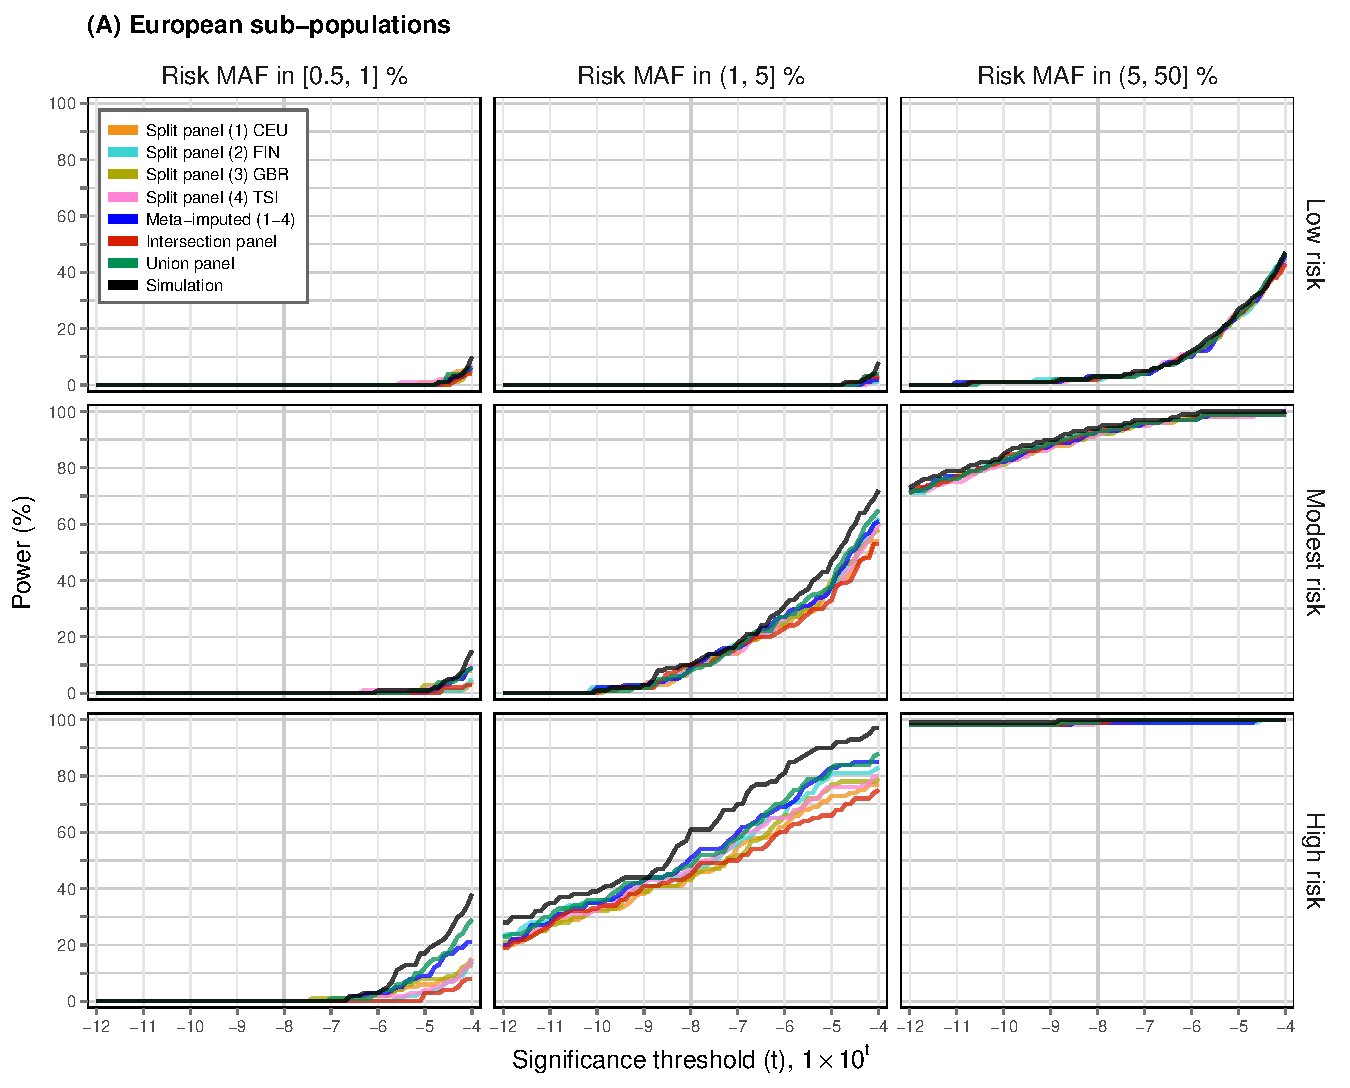
\includegraphics[width=\textwidth]{./img/ch2/association_power_A}
\Caption{Power measured under a moving significance threshold}
{Power was calculated as the proportion of replicate association analyses ($n=100$, per combination of risk category and \gls{maf} interval) in which any signal reached significance within 1~\gls{Mb} around the position of a simulated risk variant.
A moving significance threshold between ${\pvalue\leq\num{1e-8}}$ and ${\pvalue\leq\num{1e-4}}$ was applied to each association dataset.}
{fig:gwas_power_A}
\end{figure}



\begin{figure}[tb]
\ContinuedFloat
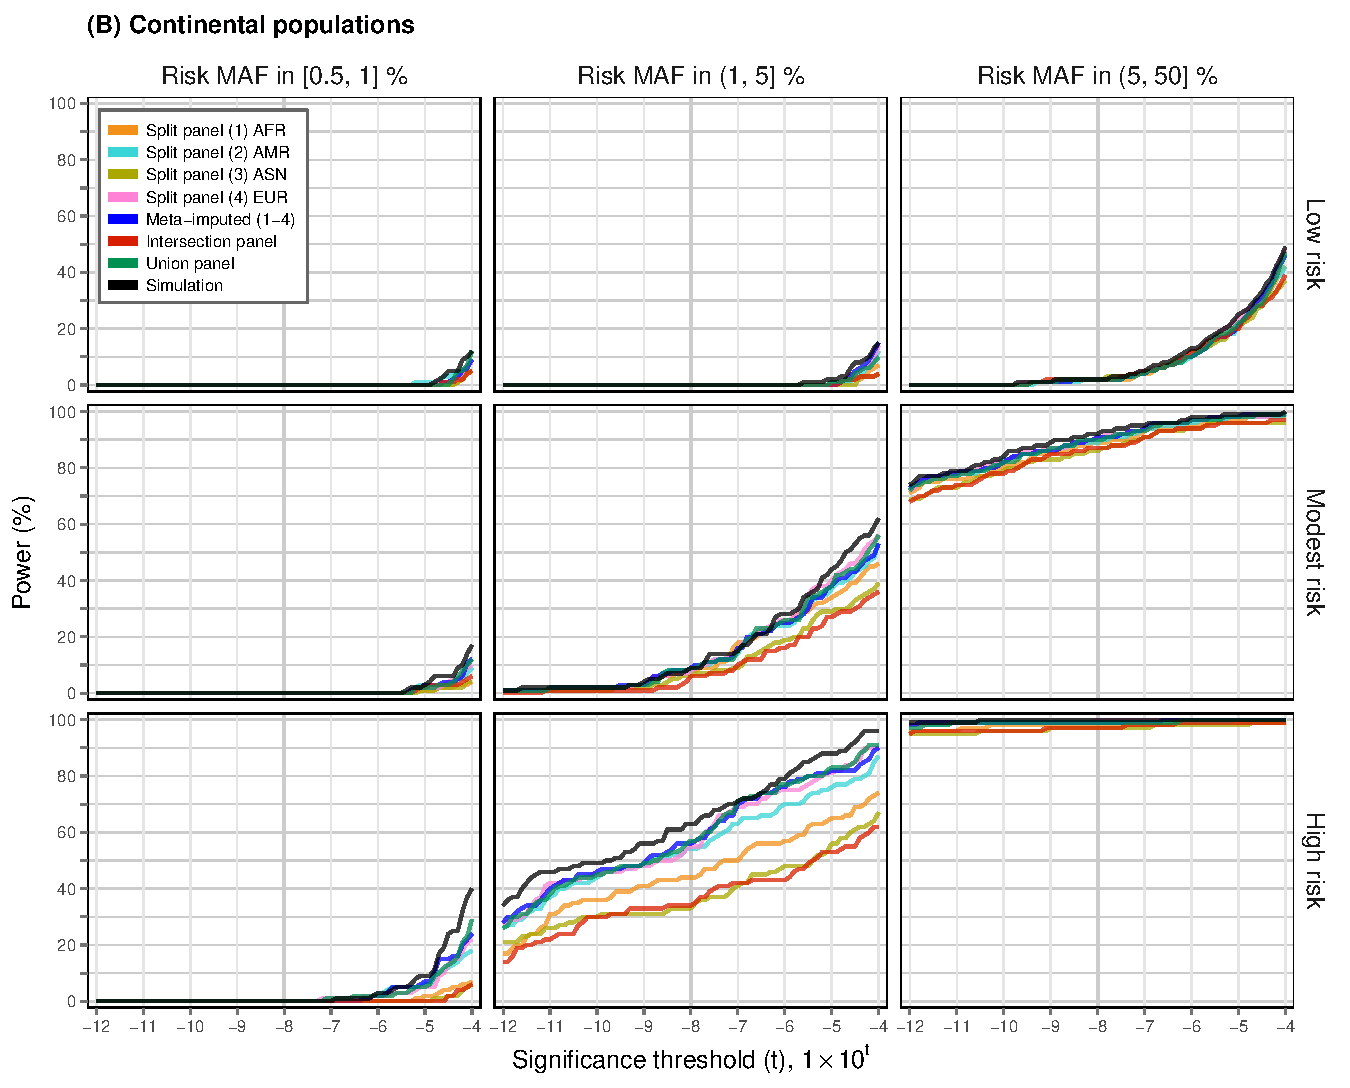
\includegraphics[width=\textwidth]{./img/ch2/association_power_B}
\caption[]{Continued.}
\label{fig:gwas_power_B}
\end{figure}



\begin{figure}[tb]
\ContinuedFloat
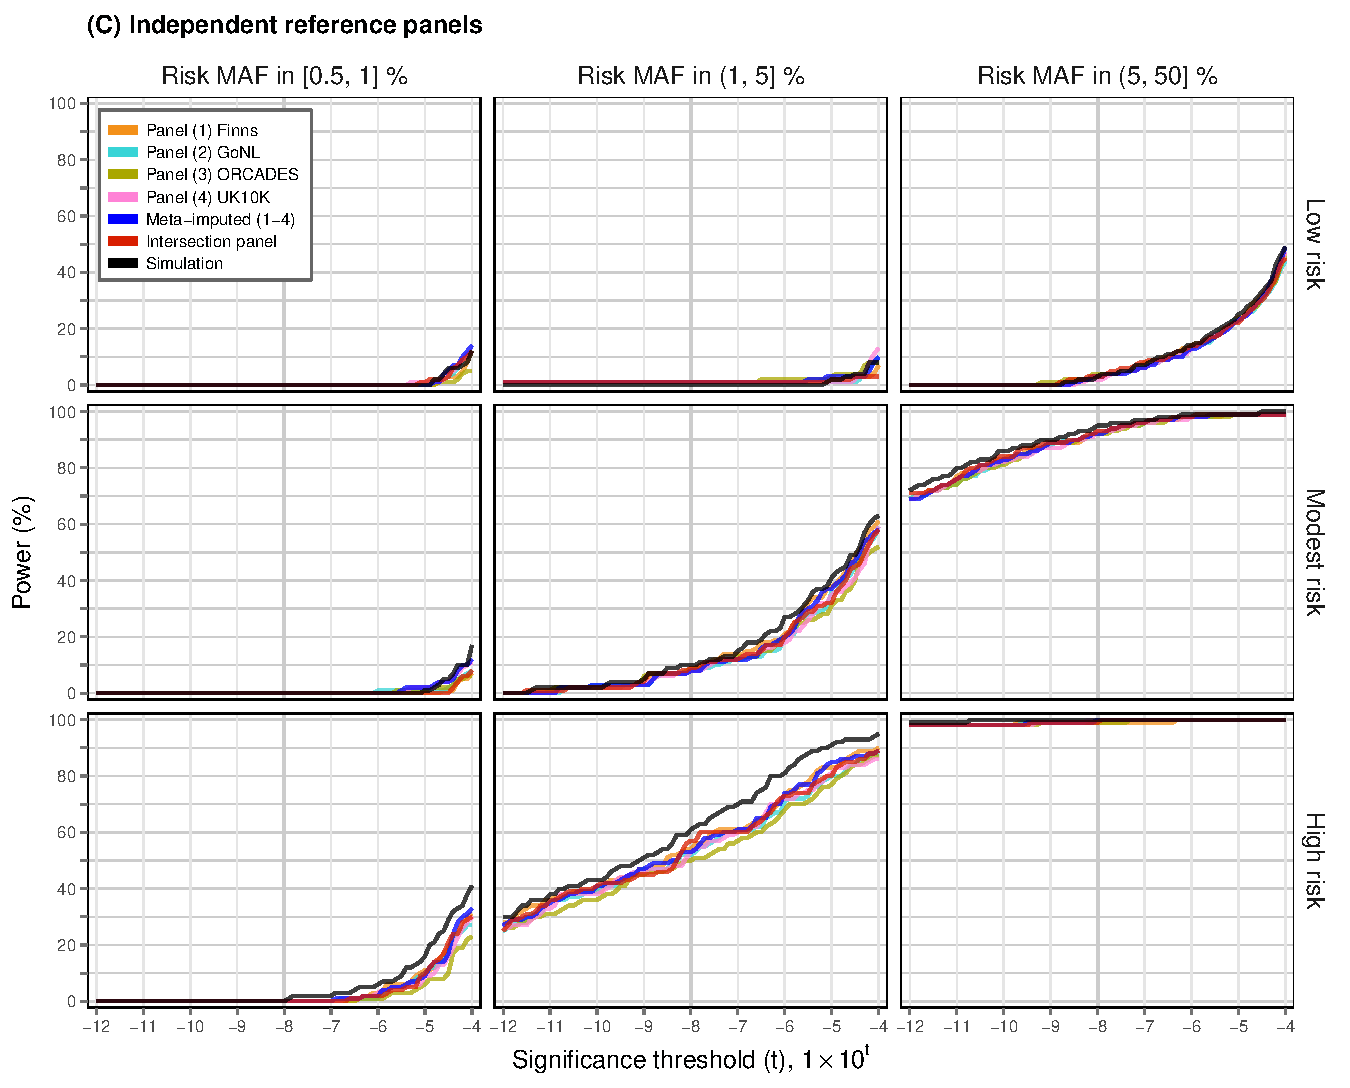
\includegraphics[width=\textwidth]{./img/ch2/association_power_C}
\caption[]{Continued.}
\label{fig:gwas_power_C}
\end{figure}
